\documentclass[14pt,a4paper,titlepage]{extarticle}
\usepackage[utf8]{inputenc}
\usepackage[english,ukrainian]{babel}
\linespread{1} %полуторный межстрочный интервал
\usepackage[pdftex,left=2cm,right=2cm,top=2cm,bottom=2cm]{geometry} %поля
\pagestyle{myheadings} %номер страниц
\usepackage{indentfirst} %чтобы абзац после названия раздела был с красной строки
\parindent=1.25cm %красная строка 1,25см
\righthyphenmin=2 %чтобы 2 последние буквы слова переносились тоже
\sloppy %выривнивание по ширине
\usepackage{amssymb}
\usepackage{amsmath}
\usepackage{verbatim}

\makeatletter 
\renewcommand{\@biblabel}[1]{#1.}
\usepackage{misccorr} %для точки после номера раздела

\usepackage[table,xcdraw]{xcolor}

\newcommand{\RomanNumeralCaps}[1]
    {\MakeUppercase{\romannumeral #1}}

\usepackage{graphicx}
\graphicspath{{pictures/}}
\DeclareGraphicsExtensions{.png,.jpg}

\begin{document}
      \begin{titlepage}
      %\thispagestyle{empty}
         \begin{center}
ДНІПРОВСЬКИЙ НАЦІОНАЛЬНИЙ УНІВЕРСИТЕТ ІМ. О. ГОНЧАРА\\
ФАКУЛЬТЕТ ПРИКЛАДНОЇ МАТЕМАТИКИ\\
КАФЕДРА КОМП'ЮТЕРНИХ ТЕХНОЛОГІЙ\\
            \vspace{6cm}
            \bf Лабораторна робота №1\\
            \bf <<НАБЛИЖЕННЯ ФУНКЦІЙ АЛГЕБРАЇЧНИМИ МНОГОЧЛЕНАМИ>>\\
            \bf з курсу <<Методи обчислень>>\\
            \bf Варіант №2
        \end{center}
        \vspace{5cm}
        \begin{flushright}
Виконав:\\
студент групи ПА-18-1(2)\\
Лєшанов Андрій
        \end{flushright}
        \begin{center}
        \vspace{5.5cm}
        Дніпро, 2020
        \end{center}
   \end{titlepage}
\setcounter{page}{2}
\newpage
{\centering\tableofcontents}
\newpage
{\centering \section*{Постановка задачі}}
\addcontentsline{toc}{section}{Постановка задачі}
Функція $y = f(x)$ задана таблицею значень в точках $x_i, i = 0, 1 \ldots n$.\\
\begin{center}


{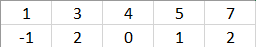
\includegraphics[scale=1]{6}}
\end{center}

Необхідно:\\
1. Побудувати інтерполяційний многочлен $L_n(x)$ за формулою Лагранжа.\\
2. Побудувати інтерполяційний многочлен $P_n(x)$ за формулою Ньютона.\\
3. За допомогою методу найменших квадратів побудувати многочлен $Q_m(x)$ степеня $m \leqslant n$\\
4. Обчислити значення кожного з поліномів $L_n(x), P_n(x), Q_m(x)$ в точках
$$
\widetilde{x}_i = x_i + \frac{h_i}{2}, де h_i = x_{i+1} - x_i, i = \overline{0, n-1}
$$
та в точках $\widetilde{x}_{-1} = x_0 - \frac{h_0}{2}$, $\widetilde{x}_n = x_n + \frac{h_{n-1}}{2}$.
Результати надрукувати у вигляді порівнялної таблиці.\\
5. Побудувати на одному графіку три залежності $y = L_n(x)$, $y = P_n(x)$, $y = Q_m(x)$ на відрізку $\left[\widetilde{x}_{-1}, \widetilde{x}_{n}\right]$. На цьому ж графіку відмітити задані таблицею точки $\left(x_i, y_i\right), i = \overline{0, n}$.\\
6. Проаналізувати поведінку поліному $Q_m(x)$ при різних степенях $m$.\\
\newpage
{\centering \section{Основні теоретичні відомості}}
{\centering \subsection{Інтерполяційна формула Лагранжа. Залишок}}
{\centering \subsection{Поділені різниці та їх властивості}}
{\centering \subsection{Інтерполяційні формули Ньютона. Залишок}}
{\centering \subsection{Середньоквадратичне наближення функцій. Похибка}}
{\centering \section{Чисельний експеримент та аналіз результатів}}
{\centering \subsection{Опис програмної реалізації}}

Для зручності програмної реалізації, спочатку опишемо такі допоміжні структури:\\
 struct poly\_node - доданок алгебраїчного многочлену, складається з полів для степеня $x$ і для коефіцієнта перед ним. Призначена для коректної роботи наступного\\
 class Polynom - структура алгербаїчного многочлену, побудована з poly\_node.\\
 struct int\_node - реалізація вузлів інтерполяції і значень функції в цих вузлах. З цих об'єктів складемо вектор для обчислення поліномів.\\
 Головні структури для обчислень:
 class Computation - абстрактний клас для обчислень поліномів.\\
 class Lagrange\_comp - клас нащадок Computation для обчислення поліному методом Лагранжа.\\
 class Newton\_comp - клас нащадок Computation для обчислення поліному методом Ньютону.\\
 class Smallest\_square - клас нащадок Computation для обчислення поліному методом найменших квадратів.\\
 На початку виконання програми будуємо вектор точок int\_node з точок, які дані в умові. З цього вектору створюємо об'єкти для обчислень. Викликаємо відповідні функції для обчислень поліномів в цих об'єктах.\\
 Об'єкти різних типів, що відповідають за обчислення різними методами, віконують свої методи по-різному. 
 Для кожного методу знаходження коефіцієнтів поліному описані окремі функції.
{\centering \subsection{Аналіз результатів}}
{\centering \section*{Висновки}}

\addcontentsline{toc}{section}{Висновки}
{\centering \section*{Перелік використанних джерел}}

\addcontentsline{toc}{section}{Перелік використанних джерел}
\newpage
{\centering \section*{Додаток. Код програми}}

\addcontentsline{toc}{section}{Додаток. Код програми}
Файл Header.h
\begin{verbatim}
#pragma once

#include <iostream>
#include <vector>
#include <cstdlib>
#include <algorithm>
#include <functional>
#include <cmath>

using namespace std;

\end{verbatim}
Файл Polynom.h
\begin{verbatim}
#pragma once
#include "Header.h"

template<typename T>
T max(T a, T b);

template<typename T>
T min(T a, T b);


struct poly_node
{
public:
	poly_node(double a, int b) : degree(b), odd(a) {}
	poly_node& operator*(poly_node a)
	{
		poly_node* res = new poly_node(*this);
		res->degree += a.degree;
		res->odd *= a.odd;
		return *res;
	}
	poly_node& operator/(poly_node a)
	{
		poly_node* res = new poly_node(*this);
		res->degree -= a.degree;
		res->odd /= a.odd;
		return *res;
	}
	bool operator>(poly_node a)
	{
		if (degree > a.degree)
			return 1;
		return 0;
	}

	bool operator<(poly_node a)
	{
		if (degree < a.degree)
			return 1;
		return 0;
	}
	bool operator>=(poly_node a)
	{
		if (degree >= a.degree)
			return 1;
		return 0;
	}
	bool operator<=(poly_node a)
	{
		if (degree <= a.degree)
			return 1;
		return 0;
	}

	//private:
	double odd;
	int degree;

};

class Polynom
{
public:
	Polynom(vector<poly_node>& nodess) : nodes(nodess)
	 { polynomial_simplification(); }
	Polynom() {}
	~Polynom();
	//Polynom& operator=(Polynom p);
	Polynom& operator+(Polynom p);
	Polynom& operator-(Polynom p);
	Polynom& operator*(Polynom p);
	void Print();
	//Polynom& operator/(Polynom p);
	Polynom& operator/(double p);
	Polynom& operator*(double p);
	friend class Computation;
	friend class Lagrange_comp;
	friend class Newton_comp;
	friend class Smallest_square;
private:



	void polynomial_simplification();
	vector<poly_node> nodes;
};


\end{verbatim}
Файл Polynom.cpp
\begin{verbatim}
#include "Polynom.h"

template<typename T>
T max(T a, T b)
{
	if (a > b)
	{
		return a;
	}
	return b;
}

template<typename T>
T min(T a, T b)
{
	if (a < b)
	{
		return a;
	}
	return b;
}



/*
Высшие степени в начале вектора

*/



	Polynom::~Polynom() { }

	/*Polynom& Polynom:: operator=(Polynom p)
	{
		nodes = p.nodes;
		degree = p.degree;
		return *this;
	}*/

	Polynom& Polynom::operator+(Polynom p)
	{
		Polynom* res = new Polynom(*this);
		for (int i = 0; i < p.nodes.size(); i++)
		{
			res->nodes.push_back(p.nodes[i]);
		}
		sort(res->nodes.begin(), res->nodes.end());
		reverse(res->nodes.begin(), res->nodes.end());
		res->polynomial_simplification();
		return *res;
	}

	Polynom& Polynom::operator-(Polynom p)
	{
		Polynom* res = new Polynom(*this);
		for (size_t i = 0; i < p.nodes.size(); i++)
		{
			p.nodes[i].odd *= -1;
		}
		return *res + p;
	}

	Polynom& Polynom::operator*(Polynom p)
	{
		Polynom* res = new Polynom;
		for (size_t i = 0; i < nodes.size(); i++)
		{
			for (size_t j = 0; j < p.nodes.size(); j++)
			{
				res->nodes.push_back(nodes[i] * p.nodes[j]);
			}
		}
		res->polynomial_simplification();
		return *res;
	}

	Polynom& Polynom::operator/(double p)
	{
		Polynom* res = new Polynom(*this);
		for (size_t i = 0; i < nodes.size(); i++)
		{
			res->nodes[i].odd /= p;
		}
		return *res;
	}

	Polynom& Polynom::operator*(double p)
	{
		Polynom* res = new Polynom(*this);
		for (size_t i = 0; i < nodes.size(); i++)
		{
			res->nodes[i].odd *= p;
		}
		return *res;
	}


	void Polynom::polynomial_simplification()
	{
		sort(nodes.begin(), nodes.end());
		reverse(nodes.begin(), nodes.end());
		if (nodes.size())
		{

		
		for (int i = 0; i < nodes.size() - 1; i++)
		{
			if (nodes[i].degree == nodes[i + 1].degree)
			{
				nodes[i].odd += nodes[i + 1].odd;
				nodes.erase(nodes.begin() + i + 1);
				if (i)
				--i;
			}
			if (nodes[i].odd == 0)
			{
				nodes.erase(nodes.begin() + i);
			}
		}
		if (nodes[nodes.size() - 1].odd == 0)
		{
			nodes.erase(nodes.end() - 1);
		}
	}
	}

	void Polynom::Print()
	{
		
		for (int i = 0; i < nodes.size() - 1; i++)
		{
			cout  << nodes[i].odd << "x^" << nodes[i].degree;
			if (nodes[i + 1].odd >= 0)
			{
				cout << " + ";
			}
			else
			{
				cout << " ";
			}
		}
		cout << nodes[nodes.size() - 1].odd 
		<< "x^" << nodes[nodes.size() - 1].degree << "\n";
	}
\end{verbatim}
Файл Interpolation.h
\begin{verbatim}
#pragma once
#include "Header.h"
#include "Polynom.h"


struct int_node
{
	double x;
	double y;
	void operator=(int_node a) { x = a.x; y = a.y; }
};

class Computation
{
protected:
	Computation(vector<int_node> interpolation_nodes);

	virtual void Polynom_calculate() = 0;
	virtual double Value_in_point(double x) = 0;

	vector<int_node> interpolation_nodes;
	int n;
	bool calculated;

};

class Lagrange_comp : public Computation
{
public:
	Lagrange_comp(vector<int_node> interpolation_nodes) :
	Computation(interpolation_nodes) {}
	virtual void Polynom_calculate();
	virtual double Value_in_point(double x);
	void Print() { if (calculated) Lag_pol.Print(); }
private:

	Polynom& l_i(int i);


	Polynom Lag_pol;
};



class Newton_comp : public Computation
{
public:
	Newton_comp(vector<int_node> interpolation_nodes) :
	Computation(interpolation_nodes) {}
	virtual void Polynom_calculate();
	virtual double Value_in_point(double x);
	void Print() { if (calculated) 
	{ New_pol_forward.Print();  New_pol_backward.Print(); } }

private:
	Polynom& Newton_poly_forward();
	Polynom& Newton_poly_backward();
	double divided_diff(vector<int_node>);
	Polynom New_pol_forward;
	Polynom New_pol_backward;
};
\end{verbatim}

Файл Interpolation.cpp
\begin{verbatim}
#include "Interpolation.h"


Computation::Computation(vector<int_node> interpolation_nodes):
	interpolation_nodes(interpolation_nodes),
	calculated(0)
{
	n = interpolation_nodes.size() - 1;
}



double Lagrange_comp::Value_in_point(double x)
{
	double res = 0;
	if (!calculated)
	{
		Polynom_calculate();
	}
	for (int i = 0; i < n; i++)
	{
		res += pow(x, Lag_pol.nodes[i].degree) * Lag_pol.nodes[i].odd;
	}
	return res;
}

Polynom& Lagrange_comp::l_i(int i)
{
	Polynom* res = new Polynom(*(new vector<poly_node>({ {1, 0} })));
	for (int j = 0; j <= n; j++)
	{
		if (j != i)
		{
			Polynom* tmp
			 = 
			new Polynom(*(new vector<poly_node>
			({ {-interpolation_nodes[j].x, 0},  {1, 1} })));
			*tmp = *tmp / (interpolation_nodes[i].x - interpolation_nodes[j].x);
			*res = *res * *tmp;
		}

	}
	return *res;
}

void Lagrange_comp::Polynom_calculate()
{
	for (int i = 0; i <= n; i++)
	{
		Lag_pol = Lag_pol + (l_i(i) * interpolation_nodes[i].y);
	}
	calculated = 1;
}


double Newton_comp::divided_diff(vector<int_node> ixys)
{
	if (ixys.size() == 2)
	{
		return (ixys[ixys.size() - 1].y - ixys[0].y)
		 / 
		(ixys[ixys.size() - 1].x - ixys[0].x);
	}
	vector<int_node> tmp1, tmp2;
	for (size_t i = 1; i < ixys.size(); i++)
	{
		tmp1.push_back(ixys[i]);
		tmp2.push_back(ixys[i - 1]);
	}
	return (divided_diff(tmp1)- divided_diff(tmp2))
	/ 
	(ixys[ixys.size() - 1].x - ixys[0].x);
}


void Newton_comp::Polynom_calculate()
{
	New_pol_forward = Newton_poly_forward();
	New_pol_backward = Newton_poly_backward();
	calculated = 1;
}

Polynom& Newton_comp::Newton_poly_backward()
{
	Polynom* result_polynom
	 = 
	new Polynom(*(new vector<poly_node>
	({ {interpolation_nodes[n].y, 0} })));
	vector<int_node> divided_diff_arg;
	divided_diff_arg.push_back(interpolation_nodes[n]);
	Polynom tmpp(*(new vector<poly_node>({ {1, 0} })));
	
	for (size_t i = n; i > 0; i--)
	{
		tmpp = tmpp 
		* 
		*(new Polynom(*(new vector<poly_node>
		({ {1, 1}, {-interpolation_nodes[i].x ,0} }))));
		divided_diff_arg.push_back(interpolation_nodes[i-1]);
		*result_polynom = *result_polynom
		 + 
		(tmpp * divided_diff(divided_diff_arg));
	}
	return *result_polynom;
}

Polynom& Newton_comp::Newton_poly_forward()
{
	Polynom* result_polynom = 
	new Polynom(*(new vector<poly_node>
	({ {interpolation_nodes[0].y, 0} })));
	vector<int_node> tmp;
	tmp.push_back(interpolation_nodes[0]);
	Polynom tmpp(*(new vector<poly_node>({ {1, 0} })));
	for (size_t i = 1; i < n + 1; i++)
	{
		tmpp = tmpp 
		* 
		*(new Polynom(*(new vector<poly_node>
		({ {1, 1}, {-interpolation_nodes[i - 1].x ,0} }))));
		tmp.push_back(interpolation_nodes[i]);
		*result_polynom = *result_polynom + (tmpp * divided_diff(tmp));
	}
	return *result_polynom;
}


double Newton_comp::Value_in_point(double x)
{
	double res = 0;
	if (!calculated)
	{
		Polynom_calculate();
	}
	for (int i = 0; i < n; i++)
	{
		res += pow(x, New_pol_forward.nodes[i].degree)
		 *
		New_pol_forward.nodes[i].odd;
	}
	return res;
}
\end{verbatim}
Файл Main.cpp
\begin{verbatim}
#include "Header.h"
#include "Interpolation.h"
#include "Polynom.h"


int main()
{
	cout.precision(25);
	vector<int_node> points({ {1,-1}, {3, 2}, {4,0}, {5,1}, {7, 2} });
	Lagrange_comp c(points);
	Newton_comp newt(points);
	c.Polynom_calculate();
	c.Print();
	newt.Polynom_calculate();
	newt.Print();
	//cout << points.size();
	return EXIT_SUCCESS;
}
\end{verbatim}
\end{document} 